%!TEX TS-program = xelatex

\documentclass[t]{beamer}

\usetheme{Hannover}
\usecolortheme{rose}

%%% Работа с русским языком
\usepackage[english,russian]{babel}   %% загружает пакет многоязыковой вёрстки
\usepackage{fontspec,xltxtra,xunicode}      %% подготавливает загрузку шрифтов Open Type, True Type и др.
%\defaultfontfeatures{Ligatures={TeX},Renderer=Basic}  %% свойства шрифтов по умолчанию
\setmainfont[Ligatures={TeX,Historic},
SmallCapsFont={Brill},
SmallCapsFeatures={Letters=SmallCaps}]{Brill} %% задаёт основной шрифт документа
\setsansfont{Brill}                    %% задаёт шрифт без засечек
\setmonofont[Ligatures=NoCommon]{DejaVu Sans}
\newfontfamily\SYM{Brill}
\usepackage{indentfirst}
%%% Дополнительная работа с математикой
\usepackage{amsmath,amsfonts,amssymb,amsthm,mathtools} % AMS
\usepackage{icomma} % "Умная" запятая: $0,2$ --- число, $0, 2$ --- перечисление

%%% Работа с картинками
\usepackage{wrapfig} % Обтекание рисунков текстом
\usepackage{rotating}
\usepackage{fixltx2e}
\usepackage{hhline}
\usepackage{lscape}

%%% Работа с таблицами
\usepackage{array,tabularx,tabulary,booktabs} % Дополнительная работа с таблицами
\usepackage{longtable}  % Длинные таблицы
\usepackage{multirow} % Слияние строк в таблице

\usepackage{multicol} % Несколько колонок
%%% Страница
%\usepackage{fancyhdr} % Колонтитулы
% 	\pagestyle{fancy}
 	%\renewcommand{\headrulewidth}{0pt}  % Толщина линейки, отчеркивающей верхний колонтитул
% 	\lfoot{Нижний левый}
% 	\rfoot{Нижний правый}
% 	\rhead{Верхний правый}
% 	\chead{Верхний в центре}
% 	\lhead{Верхний левый}
%	\cfoot{Нижний в центре} % По умолчанию здесь номер страницы

\usepackage{setspace} % Интерлиньяж
%\onehalfspacing % Интерлиньяж 1.5
%\doublespacing % Интерлиньяж 2
\singlespacing % Интерлиньяж 1

\usepackage{subfig} % подкартинки
\usepackage{lastpage} % Узнать, сколько всего страниц в документе.
\usepackage{soul} % Модификаторы начертания
\usepackage{bbding}
\usepackage{tikz} % Работа с графикой
\usepackage{pgfplots}
\usepackage{pgfplotstable}
\usepackage{verbatim}

\usepackage{attachfile2}
\usepackage{alltt}

%%% Лингвистические пакеты
%\usepackage{savetrees} % пакет, который экономит место
\usepackage{forest} % для рисования деревьев
\usepackage{vowel} % для рисования трапеций гласных
\usepackage{natbib}
\bibpunct[: ]{[}{]}{;}{a}{}{,}
\usepackage[nogroupskip,nopostdot, nonumberlist]{glossaries}
%\usepackage{glossary-mcols} 
%\setglossarystyle{mcolindex}
\usepackage{philex} % пакет для примеров
\newcommand{\mytem}{\item[$\circ$]}
\addto\captionsrussian{
\renewcommand{\refname}{}}

\newcommand{\apostrophe}{\XeTeXglyph\XeTeXcharglyph"0027\relax}
\usetikzlibrary{patterns}

\usepackage{ulem}

\usepackage{hyperref}
\hypersetup{ % Гиперссылки
	colorlinks=true, % false: ссылки в рамках; true: цветные ссылки
	linkcolor=black, % внутренние ссылки
	citecolor=black, % на библиографию
	filecolor=black, % на файлы
	urlcolor=blue % на URL
	}
\setbeamercolor{alerted text}{fg=blue}
\setbeamersize{text margin left=4mm,text margin right=1mm} 
\setbeamertemplate{frametitle}[default][center]
\setbeamertemplate{navigation symbols}{
	\usebeamerfont{footline}%
    \usebeamercolor[fg]{footline}%
    \hspace{1em}%
    {{\small presentation is available: \href{https://tinyurl.com/u25j79m}{\textbf{https://tinyurl.com/u25j79m}}}
    \hspace{4cm}
    \insertframenumber/\inserttotalframenumber\vspace{0.5mm}}}
\title[]{Phonations, Obstruents}
\author[]{G. Moroz}
\date{12 March, 2020}
\begin{document}
\frame{\titlepage}

\begin{frame}{Previously}
\begin{itemize}
\item Waves, Fourier transform, Tube model
\item Vowels
\item Sonorants
\end{itemize}
\pause
Today we are going to talk about
\begin{itemize}
\item Airostream mechanisms
\item Phonations
\item Obstruents
\end{itemize}

\end{frame}

\section{Airstream mechanisms}
\begin{frame}{Airstream mechanisms}
\begin{center}
\begin{tabular}{|l|l|l|}
\hline
 & \multicolumn{1}{c|}{egressive} & \multicolumn{1}{c|}{ingressive} \\ \hline
pulmonic & majority of sounds & \href{http://ingressivespeech.info/}{rare} \\ \hline
glottalic & \href{http://wals.info/feature/7A\#2/13.6/152.9}{ejectives} & \href{http://wals.info/feature/7A\#2/13.6/152.9}{implosives} \\ \hline
velaric &  & \href{https://www.youtube.com/watch?v=31zzMb3U0iY}{clicks}\\ \hline
\end{tabular}
\end{center} 

\href{http://www.seeingspeech.ac.uk/ipachart/display.php?chart=2\&datatype=1\&speaker=1}{Here} is some MRI video.
\end{frame}

\section{Phonation}
\begin{frame}{\href{https://www.youtube.com/watch?v=FG_iE0FdXRk}{Phonation types}}
\begin{description}
\item[\href{https://www.youtube.com/watch?v=v9Wdf-RwLcs}{Modal voice}] --- the vocal folds are closed during half of each glottal cycle and open during the other half (approximately). Thus, the proportion of time that the glottis is open (the open quotient) during each cycle is 0.5.
\item[\href{https://www.youtube.com/watch?v=BYSZS1LaABQ}{Creaky voice}] --- the vocal folds are held together loosely, and air bubbles up through them. This cause longer closed phase of the glottal period and a comparably shorter open phase (and thus a smaller open quotient).
\item[\href{https://www.youtube.com/watch?v=9cKnUFZjs8k}{Breathy voice}] --- the vocal folds vibrate, but without much contact (for some people the vocal folds do not completely close during breathy voicing). So the glottis is open for a relatively long portion of each glottal cycle.
\end{description}
A device called an \href{http://splab.net/APD/G100/G100_01.webm}{artificial larynx} is often used as a prosthesis for patients who have had their larynx removed due to disease.
\end{frame}

\begin{frame}{Phonation types}
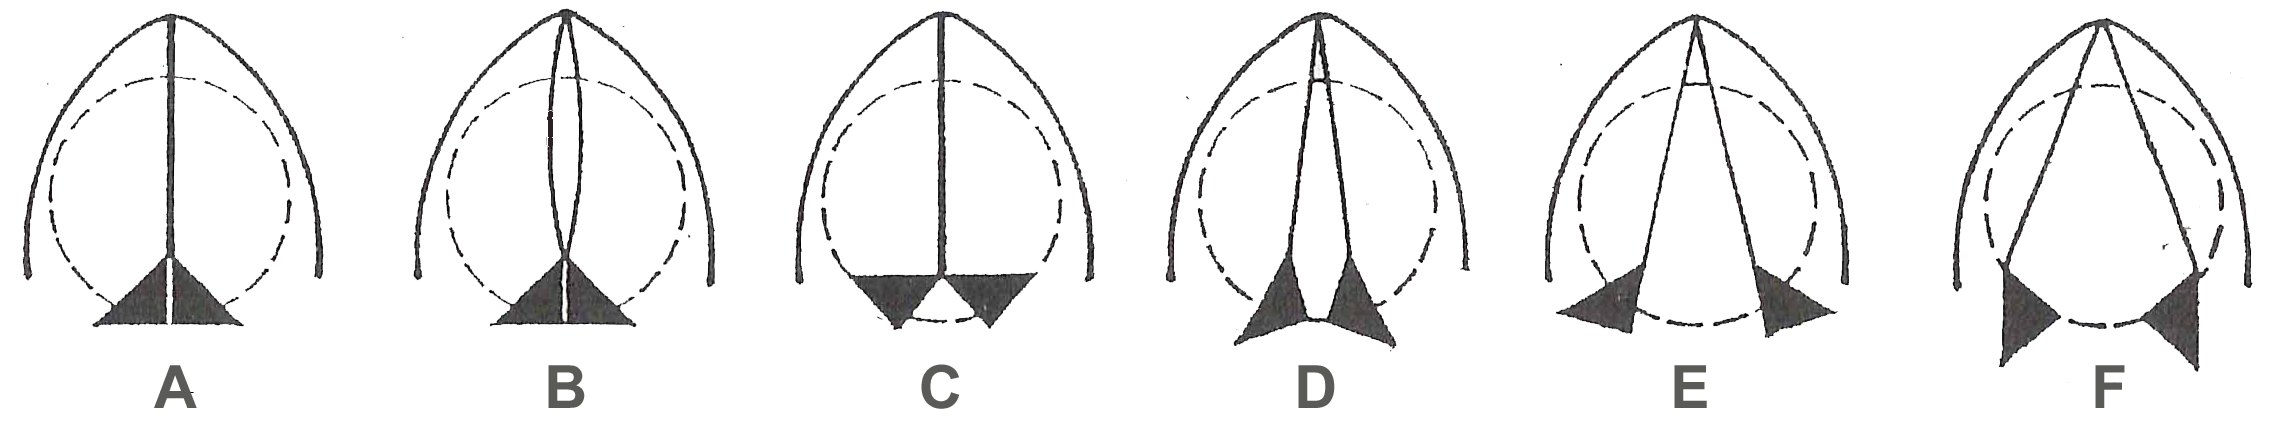
\includegraphics[width=\linewidth]{01-glottis-positions.png}
\begin{itemize}
\item[A] the closed vocal folds produce a \textbf{glottal stop ʕ}
\item[B] the air forced through the closed vocal folds produce \textbf{creaky voice}
\item[C]  air can go through vocal folds without extra pressure, making them vibrate, this is called \textbf{modal voice}
\item[D] high rate of airflow makes vocal folds vibrate even if they are slightly pulled apart (\textbf{breathy voice})
\item[E]  pulling the vocal folds further apart doesn't allow them vibrate, the result is a \textbf{voiceless sound}
\item[F] pull the vocal fold further apart, this is called \textbf{aspiration}
\end{itemize}
\end{frame}

\begin{frame}{Phonation types}
In \citep{ladefoged71} it is suggested that there might be a continuum of phonation types:\\
\begin{center}
\begin{tabular}{ccccc}
\textbf{most open} & \multicolumn{3}{c}{$\xleftrightarrow{\hspace*{3.5cm}}$}  & \textbf{most closed} \\
voiceless & breathy & modal & creaky & glottal closure \\ 
\end{tabular}
\end{center}
\end{frame}

\begin{frame}{Phonation types}
As a consequence of noise in breathy phonation, there is much more
aperiodic energy across the spectrum and the formant structure is less clear \citep{gordon01}
\begin{center}
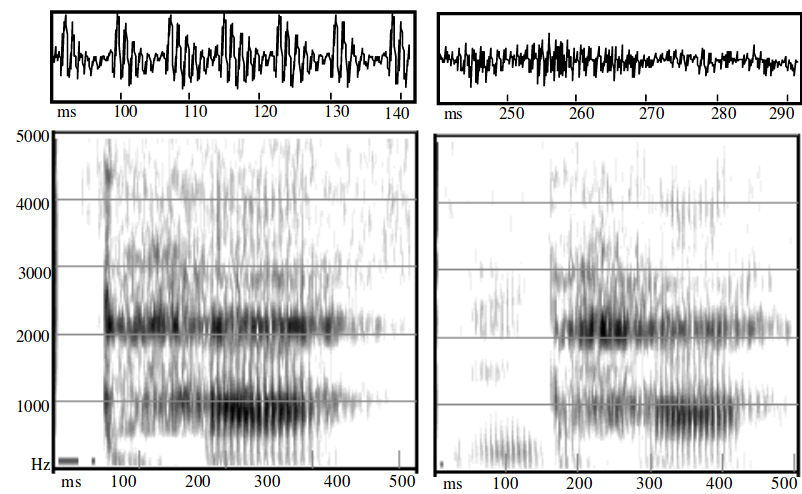
\includegraphics[width=0.73\linewidth]{02-breathy.png}
\end{center}
Spectrograms of modal and breathy voiced nasals in the Jalapa Mazatec  words /ntʰǽ/ ‘seed’ and /ndǽ̰/ ‘horse’ (female speaker)\\
\end{frame}

\begin{frame}{Phonation types}
Creaky phonation is characterized with irregular glottal periods (jitter) but
with clear formant structure. As a consequence of this irregularity, F$_0$
is not (usually) calculated so accurately.
\begin{center}
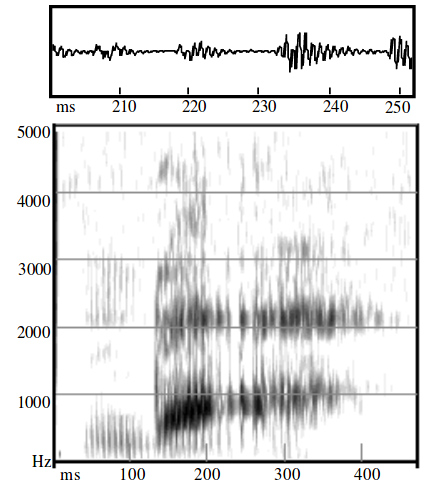
\includegraphics[width=0.40\linewidth]{03-creaky.png}
\end{center}
Spectrograms of modal and breathy voiced nasals in the Jalapa Mazatec  word /ndǽ/ ‘horse’ (female speaker)\\
\end{frame}
\section{Obstruents}
\begin{frame}{Obstruents}
\small
\vspace{-0.5cm}
\begin{forest}
where n children = 0{tier = word}{}
[Consonants,  for tree={parent anchor=east, child anchor=west, grow=0}
 [Sonorants
  [Nasals [{m, n, …}]]
  [Approximants
    [Lateral [{l, ɭ, ...}]]
    [Central [{j, w, ɹ ...}]]]
  [Trill/tap [{r, ɾ, ʀ, ...}]]]	
  [Obstruents
    [Stops 
      [{b, t, ɡ, q, ...}]]
    [Fricatives 
      [Sibilant [{s, ʃ, ...}]] 
      [{f, θ, ɦ, ...}]]
    [Affricates 
      [Sibilant [{ts, dʒ, ...}]] 
      [{pf, qχ, ...}]]]]
\end{forest}
\normalsize\\
For obstruents the articulators form constrictions and occlusions within the vocal tract that generate \textbf{aperiodic noise} as the airflow passes through obstructions: \hspace*{\fill} much more restricted airflow; \\
\hspace*{\fill} acoutically, little or no of formant structure\\
\end{frame}
\subsection{Fricatives}
\begin{frame}{Torbulence}
The main factors that determine whether airflow is turbulent: 
\begin{itemize}
\item the size of the channel and 
\item the volume velocity of the airflow (volume of air going past a certain point per unit time).
\end{itemize}
If 100 cm$^3$ per second of air flows through a channel, turbulent airflow is created if the channel area is less than 10 mm$^2$, but not if the channel area is 20 mm$^2$.
It’s easier to get turbulent airflow from a narrow straw than a wide one
\end{frame}
\begin{frame}{Fricatives}
\begin{itemize}
\item sibilant are most intensive fricatives vs. non-sibilant
\item for sibilants 
\begin{itemize}
\item the constriction between the alveolar ridge, or in the postalveolar area and the tip of the tongue, or the blade of the tongue
\item a second constriction between the upper and lower incisors must be narrow so that the airstream is directed over the edges of the teeth, creating turbulent airflow behind the teeth
\end{itemize}
\item for non-sibilants noice is not so prominent, hardly audible
\end{itemize}
\end{frame}
\begin{frame}{Fricatives}
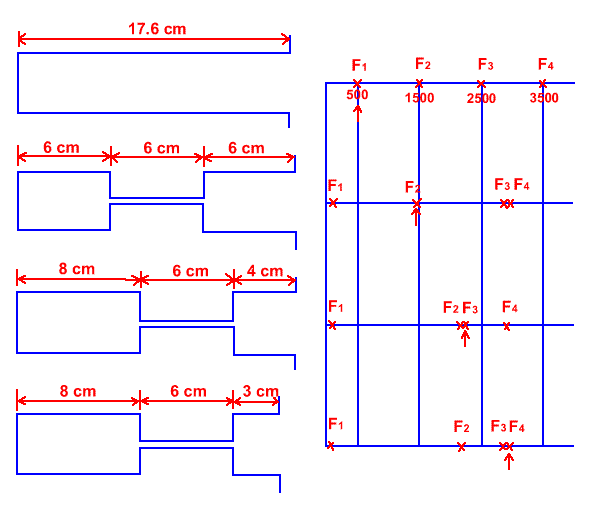
\includegraphics[width=0.7\linewidth]{04-tube.png}\\
This diagram shows the results for some models of velar and palatal consonants compared to a single tube model of a neutral vowel. (adapted from \cite[73]{fant60})
\end{frame}

\subsection{Stops}
\begin{frame}{Stops}
\begin{itemize}
\item The main articulatory posture during a stop is complete closure of the vocal tract, acoustically silence. 
\item However, languages use a great variety of stops, utilizing different places of articulation, stop release sounds, and accompanying noises
\end{itemize}
\end{frame}
\section{}
\begin{frame}
{\huge Thank you!\bigskip\\
\normalsize Please, don't hesitate to write me\\
agricolamz@gmail.com
\vspace{-130pt}}
\end{frame}
\begin{frame}{Reference}
\footnotesize
\bibliographystyle{chicago}
\bibliography{bibliography}
\end{frame}
\end{document}
